\documentclass[a4paper]{article} 
\usepackage{float}
\usepackage{grffile}
\usepackage{graphicx}
\usepackage{amssymb}
\usepackage{fontspec}
\usepackage{fancyhdr}
\usepackage{multicol}
\usepackage{calc}
\usepackage{lettrine}
\usepackage{alphalph}
\usepackage[left=2cm,right=2cm,top=1.99cm,bottom=1.99cm,includeheadfoot]{geometry}
\usepackage{changepage}
\usepackage{needspace}
\usepackage{bidi} 

\parindent=0pt
\parskip=\medskipamount
\begin{document}
\pagestyle{plain}
\sloppy
\setlength{\parfillskip}{0pt plus 1fil}
\font\letHeaddicBody="Times New Roman" at 12pt
\font\letterletHeaddicBody="Gautami/B" at 24pt
\font\letDatadicBody="Times New Roman" at 12pt
\font\entryletDatadicBody="Times New Roman" at 10pt
\font\pictureRightentryletDatadicBody="Times New Roman" at 10pt
\font\picturepictureRightentryletDatadicBody="Times New Roman" at 10pt
\font\pictureCaptionpictureRightentryletDatadicBody="Times New Roman" at 10pt
\font\CmPicturepublishStemPileThumbnailPubpictureCaptionpictureRightentryletDatadicBody="Times New Roman" at 10pt
\font\pictureLabelenpictureCaptionpictureRightentryletDatadicBody="Times New Roman" at 10pt
\font\spanenpictureLabelenpictureCaptionpictureRightentryletDatadicBody="Times New Roman" at 10pt
\font\headwordggoTeluxINentryletDatadicBody="Gautami" at 10pt
\font\pronunciationsentryletDatadicBody="Times New Roman" at 10pt
\font\pronunciationggofonipaxemicpronunciationsentryletDatadicBody="Tahoma" at 10pt
\font\spanggofonipaxemicpronunciationggofonipaxemicpronunciationsentryletDatadicBody="Tahoma" at 10pt
\font\sensesentryletDatadicBody="Times New Roman" at 10pt
\font\sensesensesentryletDatadicBody="Times New Roman" at 10pt
\font\grammaticalinfosensesensesentryletDatadicBody="Times New Roman" at 10pt
\font\partofspeechengrammaticalinfosensesensesentryletDatadicBody="Times New Roman" at 10pt
\font\spanenpartofspeechengrammaticalinfosensesensesentryletDatadicBody="Times New Roman" at 10pt
\font\xsensenumbersensesentryletDatadicBody="Times New Roman" at 10pt
\font\definitionensensesensesentryletDatadicBody="Times New Roman" at 10pt
\font\spanendefinitionensensesensesentryletDatadicBody="Times New Roman" at 10pt
\font\LexSensepublishStemGlossPubensensesensesentryletDatadicBody="Times New Roman" at 10pt
\font\spanenLexSensepublishStemGlossPubensensesensesentryletDatadicBody="Times New Roman" at 10pt
\font\examplessensesensesentryletDatadicBody="Times New Roman" at 10pt
\font\exampleggoTeluxINexamplessensesensesentryletDatadicBody="Gautami" at 10pt
\font\spanggoTeluxINexampleggoTeluxINexamplessensesensesentryletDatadicBody="Gautami" at 10pt
\font\translationsexamplessensesensesentryletDatadicBody="Times New Roman" at 10pt
\font\translationentranslationsexamplessensesensesentryletDatadicBody="Times New Roman" at 10pt
\font\xitementranslationentranslationsexamplessensesensesentryletDatadicBody="Times New Roman" at 10pt
\font\spanenxitementranslationentranslationsexamplessensesensesentryletDatadicBody="Times New Roman" at 10pt
\font\xitemtetranslationentranslationsexamplessensesensesentryletDatadicBody="Gautami" at 10pt
\font\spantexitemtetranslationentranslationsexamplessensesensesentryletDatadicBody="Gautami" at 10pt

\pagestyle{fancy} 
\begin{center}
\section*{\needspace {8\baselineskip}{\topskip 18pt{\letterletHeaddicBody{అ}}}}\end{center}

\hangindent= 36pt
\hangafter=1

\begin{wrapfigure}
\begin{center}
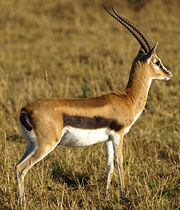
\includegraphics[angle=0,width=150mm,height=175mm]{c.jpg} 
\caption{}
\end{center}
\end{wrapfigure}



\spanenpictureLabelenpictureCaptionpictureRightentryletDatadicBody{rice with tumeric}



\hangindent= 36pt
\hangafter=1\markboth{ \headwordggoTeluxINentryletDatadicBody అక్సెదంగ్}{ \headwordggoTeluxINentryletDatadicBody అక్సెదంగ్}\headwordggoTeluxINentryletDatadicBody{అక్సెదంగ్}\spanggofonipaxemicpronunciationggofonipaxemicpronunciationsentryletDatadicBody{aksedaṅg}\spanenpartofspeechengrammaticalinfosensesensesentryletDatadicBody{n}\xsensenumbersensesentryletDatadicBody{1}\spanendefinitionensensesensesentryletDatadicBody{rice with vermilion}\spanenLexSensepublishStemGlossPubensensesensesentryletDatadicBody{rice with vermilion}\xsensenumbersensesentryletDatadicBody{2}\spanendefinitionensensesensesentryletDatadicBody{rice mixed with vermilion thrown at a wedding, or on cattle (e.g. during 'laxmi pooja') in order to bless.}\spanenLexSensepublishStemGlossPubensensesensesentryletDatadicBody{rice with turmeric used to bless}\spanggoTeluxINexampleggoTeluxINexamplessensesensesentryletDatadicBody{గొవుర్ దన్ గోటమ్నె నొవ్రి నొవ్రనగ సమ్దిర్ అక్సెదాంగ్ వాటంతెర్.}\spanenxitementranslationentranslationsexamplessensesensesentryletDatadicBody{At the wedding place, everyone throws rice on the bride andgroom.}\spantexitemtetranslationentranslationsexamplessensesensesentryletDatadicBody{$\sharp$పెండ్లి పందిరిలో పడుసు, వరులకు పసుపు బియ్యం వేస్తారు.}

\end{document}
